% !TeX root = bericht.tex
\section{Einleitung}
Dieser Bericht behandelt den zweiten Versuch des Labores Regelungstechnik. Es soll eine Füllstandsregelung in \textit{Matlab/Simulink} simuliert werden. Zwei Szenarien werden unterschieden: ein Behälter mit Zufluss aber ohne Abfluss und ein Behälter mit Zufluss und Abfluss. Für das zweite Szenario werden unterschiedliche Modelle betrachtet, um den Zusammenhang zwischen Zufluss und Abfluss mathematisch zu beschreiben.

\section{Aufgaben zur Vorbereitung}
\subsection{Mathematischer Zusammenhang zwischen Zufluss und Füllstand}
Der Behälter ist zylindrischer Form und hat eine kreisrunde Querschnittsfläche $A$ in $[m²]$ mit dem Durchmesser $d$ in $[m]$. Die Regelgröße ist der Füllstand $h(t)$ in $[m]$. Der Zufluss ist $q_{zu}(t)$ in $[\frac{m^3}{s}]$
\\
Für den Behälter ohne Abfluss gilt folgender mathematischer Zusammenhang:

\begin{equation}
    \dot{h}(t) = \frac{1}{A} \cdot q_{zu}(t) \quad 
    \Longrightarrow 
    \quad 
    h(t) = \frac{1}{A} \int q_{zu}(t) dt
\end{equation}

\subsection{Übertragungsfunktion}
Die Laplace-Transformation der Gleichung (1) ergibt die Übertragungsfunktion $G(s)$. Der Zusammenhang der Funktionen im Laplace-Bereich ist in Abbildung \ref{fig:signalfluss} dargestellt.
\begin{equation}
    G(s) = \frac{H(s)}{Q_{zu}(s)} = \frac{\mathcal{L}\{h(t)\}}{\mathcal{L}\{q_{zu}(t)\}} = \frac{1}{As} \cdot  \frac{Q_{zu}(s)}{Q_{zu}(s)} = \frac{1}{As}
\end{equation}

\begin{figure}[ht]
    \centering
    \begin{tikzpicture}[
        block/.style={rectangle, draw, thick, minimum width=2cm, minimum height=1cm, align=center},
        arrow/.style={-{Stealth[length=3mm]}, thick}
    ]
        % Eingang
        \node (input) at (-3,0) {$Q_{zu}(s)$};
        
        % Übertragungsfunktion Block
        \node [block] (G) at (0,0) {$G(s)$};
        
        % Ausgang
        \node (output) at (3,0) {$H(s)$};
        
        % Pfeile
        \draw [arrow] (input) -- (G);
        \draw [arrow] (G) -- (output);
    \end{tikzpicture}
    \caption{Signalflussdiagramm der Übertragungsfunktion $G(s)$}
    \label{fig:signalfluss}
\end{figure}

\subsection{Blockschaltbild}
Diese Übertragungsfunktion kann in einem Blockschaltbild dargestellt werden, wobei der Eingang $q_{zu}(t)$ durch einen Integrator mit der Verstärkung $\frac{1}{A}$ zum Ausgang $h(t)$ führt. Die Regelgröße ist die gewünschte Füllhöhe $h_{soll}(t)$, die mit der tatsächlichen Füllhöhe $h(t)$ verglichen wird, um den Fehler zu berechnen. Der Fehler wird von dem Regler verarbeitet, um die Stellgröße $q_{zu}(t)$ anzupassen und die gewünschte Füllhöhe zu erreichen. Das Blockschaltbild ist Grundlage für das Modell in \textit{Simulink}, welches in Abbildung \ref{blockschaltbild} gezeigt ist.

\begin{figure}[H]
    \centering
    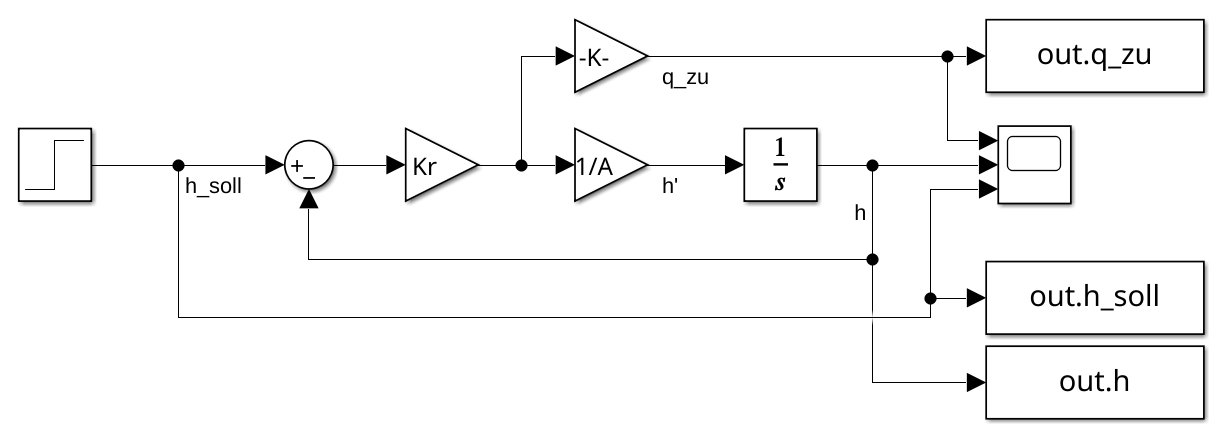
\includegraphics[width=0.9\textwidth]{graphix/modell_ohne_abfluss}
    \caption{Blockschaltbild (Screenshot aus \textit{Simulink})}
    \label{blockschaltbild}
\end{figure}

\subsection{Stationäre Genauigkeit ohne Abfluss}
Stationäre Genauigkeit bedeutet, dass die Regelgröße gegen den Sollwert konvergiert. Eine stationär genaue Regelung ist in der Lage, den Sollwert zu erreichen und zu halten. Es muss folgener mathematischer Zusammenhang gelten, damit die stationäre Genauigkeit erreicht wird:

\begin{equation}
    \lim_{t \to \infty} (h_{soll}(t)) = \lim_{t \to \infty} (h(t))
\end{equation}

Mit Zufluss und ohne Abfluss wird die Füllhöhe kontinuierlich steigen, sie kann nicht stationär genau sein. Mathematisch betrachtet würde in diesem Fall der Regelgröße divergieren. In der Realität würde die Füllhöhe steigen, bis der Behälter überläuft.

%Rechnung

\subsection{Stationäre Genauigkeit mit Abfluss}
In diesem Fall kann der Regler stationäre Genauigkeit erreichen. Wenn die einzuregelnde Füllhöhe überschritten wird, kann das Ventil des Abflusses geöffnet werden und die Füllhöhe sinkt wieder.

%Rechnung
